\section{\acl{RL} dan \textit{Q-Learning}}

Subbab ini akan menjelaskan secara detail tentang dua hal yang menjadi subjek utama dalam penelitian ini, yaitu \acl{RL} dan \textit{Q-Learning} sebagai sebuah metode yang dapat digunakan untuk membangun sebuah agen otonom.

\subsection{\acl{RL}}
\label{sub:sub-rl}

\acf{RL} merupakan sebuah kerangka pembelajaran sebuah kerangka pengembangan sebuah agen otonom yang dapat membuat suatu keputusan dalam ruang lingkup permasalahan yang terbatas. Secara umum, berikut merupakan formulasi sederhana dari kerangka \ac{RL}.

\vspace{-12mm}
\begin{flalign}
	\pi(s,a)^* = argmax(V(s,a)) &  &
\end{flalign}
\vspace{-12mm}

\(\pi\) merupakan notasi dari hasil fungsi kebijakan (\textit{policy}) yang merupakan keluaran dari \ac{RL}. Terdapat dua input untuk fungsi kebijakan tersebut, yaitu state (\(s\)) dan aksi (\(\alpha\)). Hasil yang diinginkan dari fungsi tersebut, adalah didapatkannya aksi yang terbaik dengan hasil evaluasi sebuah fungsi penilai (\(V\)). Berikut merupakan contoh dari penggunaan \ac{RL} pada gambar \ref{fig:ilustrasi-RL} sebagai ilustrasi cara kerja fungsi kebijakan.

\begin{figure}[h]
	\centering
	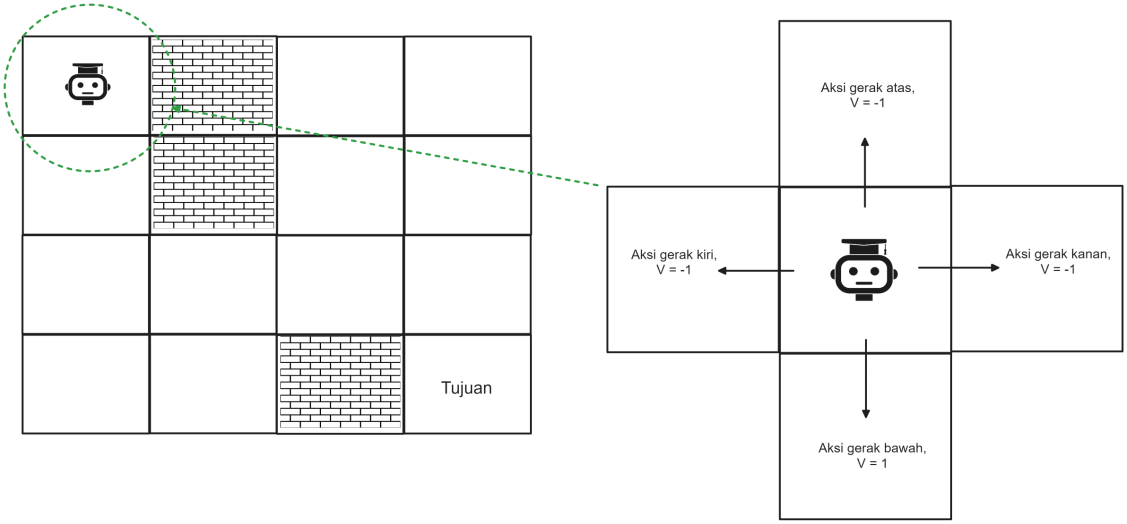
\includegraphics[width=0.8\textwidth]{chapter-2/ilustrasi-RL.png}
	\caption{Ilustrasi \ac{RL}}
	\label{fig:ilustrasi-RL}
\end{figure}


Pada gambar \ref{fig:ilustrasi-RL}, tergambarkan sebuah ilustrasi agen otonom yang berada pada sebuah konfigurasi labirin. Pada setiap posisi (\textit{state}), terdapat empat aksi yang dapat diambil oleh agen otonom tersebut: gerak kanan, gerak kiri, gerak atas, dan gerak bawah. Masing-masing aksi akan memiliki sebuah nilai yang diberikan oleh fungsi \(V\). Pada contoh Gambar \ref{fig:ilustrasi-RL}, nilai fungsi \(V\) ketika agen berjalan menuju tempat kosong akan bernilai 1 dan akan bernilai -1 untuk sebaliknya. Fungsi kebijakan pada \ac{RL}, akan meninjau nilai hasil fungsi \(V\) berdasarkan masukan seluruh aksi pada posisi tersebut dan akan memilih aksi yang menghasilkan nilai fungsi \(V\) terbesar. Pada kasus diatas, Gambar \ref{fig:ilustrasi-RL}, aksi yang akan diambil adalah aksi gerak bawah. Berdasarkan ilustrasi tersebut, dapat diperhatikan bahwa fungsi \(V\) merupakan

Pada kasus diatas, gambar 2.1, aksi yang akan diambil adalah aksi gerak bawah. Berdasarkan ilustrasi tersebut, dapat diperhatikan bahwa fungsi \(V\) merupakan esensi dari pengembangan agen \ac{RL} yang mumpuni. Fungsi \(V\) yang optimal, akan menghasilkan agen \ac{RL} yang optimal. Konstruksi fungsi \(V\) dapat dilakukan dengan berbagai metode. Pada sistem yang sederhana, fungsi \(V\) bahkan dapat diatur secara manual oleh pengembang sistem. Namun, agar fungsi \(V\) tersebut dapat berubah secara dinamik, mengikuti konfigurasi state yang mungkin berubah, agen \ac{RL} dapat dilatih menggunakan metode \textit{Q-Learning}.

\subsection{\textit{Q-Learning}}
\textit{Q-Learning} merupakan sebuah metode yang dapat digunakan untuk melakukan konstruksi fungsi penilai yang optimal untuk membangun fungsi kebijakan pada \ac{RL}. \textit{Q-Learning} menggunakan algoritma yang marak digunakan pada pengembangan agen \ac{RL} karena merupakan algoritma yang memiliki konvergensi yang stabil \parencite{lim2022regularized}. Cara kerja \textit{Q-Learning} dapat dirangkum menggunakan persamaan berikut.

\vspace{-12mm}
\begin{flalign}
	\label{eq:q-learning}
	Q_{new}(s_t,a_t) = (1-\alpha) Q(s_t, a_t) + \alpha (r_t + \gamma \cdot maxQ(s_{t+1},a)) &  &
\end{flalign}
\vspace{-12mm}

\(Q\) merupakan alternatif bentuk fungsi \(V\) yang memiliki dimensi terbatas, sebesar banyaknya aksi \(\times\) banyaknya \textit{state}. \(Q\) sering dilihat sebagai sebuah \textit{lookup table}, disebut \textit{Q-Table}, yang memiliki nilai diskrit untuk posibilitas keluaran nilai aksi berdasarkan \textit{state} terkini. Berikut, pada gambar \ref{fig:ilustrasi-qtable}, merupakan ilustrasi dari \textit{Q-Table}.

\begin{figure}[h]
	\centering
	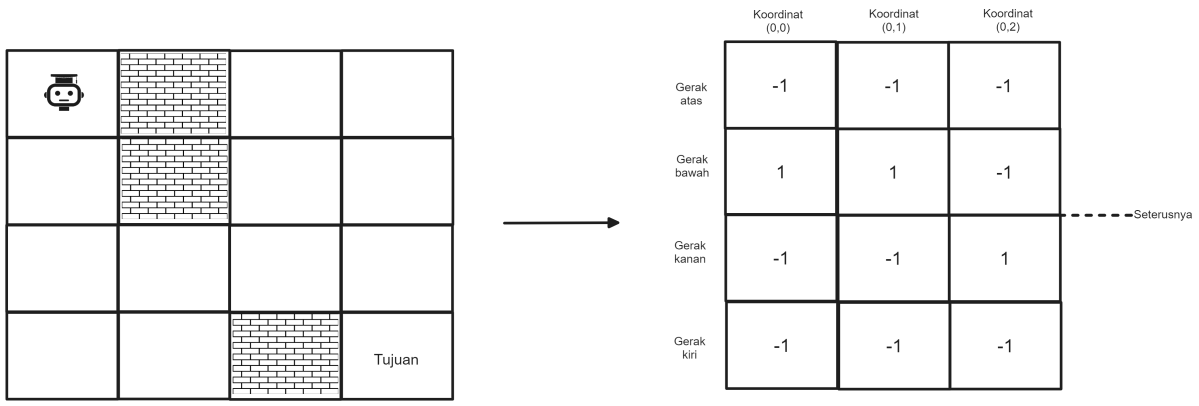
\includegraphics[width=1\textwidth]{chapter-2/ilustrasi-qtable.png}
	\caption{Ilustrasi \textit{Q-Table}}
	\label{fig:ilustrasi-qtable}
\end{figure}

Pada ilustrasi gambar \ref{fig:ilustrasi-qtable}, \textit{Q-Table} merupakan representasi hasil translasi seluruh \textit{state} (dalam bentuk koordinat) beserta seluruh aksi yang menghasilkan sebuah tabel pencarian yang dapat menghasilkan keluaran fungsi penilai dengan hanya index dari tabel tersebut menggunakan \textit{state} dan aksi.

Dengan representasi tersebut, Persamaan 2.2 dapat dipahami sebagai pembaruan nilai \textit{Q-Table} pada index (\(s\), \(a\)) dengan beberapa proporsi nilai \textit{Q-Table} sebelumnya, ditambah dengan penjumlahan dari keluaran fungsi penilai saat itu dan fungsi penilai setelah pengambilan fungsi tersebut. Berikut merupakan detail dari penjelasan tersebut.


\begin{enumerate}
	\item \((1-\alpha) Q(s_t,a_t)\): merupakan nilai \textit{Q-Table} yang akan diupdate, namun informasinya masih digunakan untuk mendapatkan nilai yang optimal sesuai dengan prinsip \textit{Markov Decision Process} \parencite{littman1994markov}.
	\item \(\alpha (r_t + \gamma \cdot maxQ(s_{t+1},a))\): merupakan nilai pembaruan \textit{Q-table} yang berasal dari keluaran fungsi penilai aksi pada state sekarang (\(r_t\)) dan sedikit kontribusi (bergantung \(\gamma\)) dari prediksi fungsi penilai pada state selanjutnya \(maxQ(s_{t+1},a)\).
\end{enumerate}

